% ****** Start of file aipsamp.tex ******
%
%   This file is part of the AIP files in the AIP distribution for REVTeX 4.
%   Version 4.1 of REVTeX, October 2009
%
%   Copyright (c) 2009 American Institute of Physics.
%
%   See the AIP README file for restrictions and more information.
%
% TeX'ing this file requires that you have AMS-LaTeX 2.0 installed
% as well as the rest of the prerequisites for REVTeX 4.1
%
% It also requires running BibTeX. The commands are as follows:
%
%  1)  latex  aipsamp
%  2)  bibtex aipsamp
%  3)  latex  aipsamp
%  4)  latex  aipsamp
%
% Use this file as a source of example code for your aip document.
% Use the file aiptemplate.tex as a template for your document.
\documentclass[%
 aps,
 amsmath,amssymb,
%preprint,%
 reprint,%
%author-year,%
%author-numerical,%
 twocolumn
]{revtex4-1}

\usepackage{graphicx}% Include figure files

\usepackage{bm}% bold math
%\usepackage[mathlines]{lineno}% Enable numbering of text and display math
%\linenumbers\relax % Commence numbering lines

\begin{document}

%\preprint{AIP/123-QED}

\title[]{Analysis of Logistic Regression and Linear Discriminant Analysis for Breast Cancer Diagnosis and Red Wine Quality}% Force line breaks with \\

\author{Tianzhu Fu}
\author{Xingyu Li}%
\author{Wenzong Xia}

\date{\today}% It is always \today, today,
             %  but any date may be explicitly specified

\begin{abstract}
\textbf{Abstract}: In this project, we investigated the performance of linear classification models on two benchmark datasets: logistic regression using gradient descent and linear discriminant analysis (LDA) to the tasks of predicting breast cancer tumor types and red wine quality. We found that the logistic regression approach was achieved worse accuracy than LDA and was significantly slower to train. We also demonstrate how gradient descent hyperparameters affect convergence rate and the quality of the obtained results. 
\end{abstract}
\maketitle
\raggedbottom

\section{Introduction}
\subsection*{\label{sec:level2}Task Description}
In this work, we implemented both logistic regression with gradient descent and linear discriminant analysis (LDA) methods and compare their performance in terms of prediction accuracy and CPU runtime. We also demonstrate how various hyperparameters can impact the convergence speed and the performance of the gradient descent variant. \par

In particular, we study the process of applying logistic regression with gradient descent and LDA to predicting tumor types (benign or malignant) based on various diagnosis information as well as predicting the red wine quality (binary) based on various properties. Details of the peculiarities of the datasets and preprocessing process for the datasets are further discussed in section III.

\subsection*{Previous Work}


\section{\label{sec:level1}Datasets}
\subsection*{\label{sec:level2}Breast Cancer Dataset}
The original breast cancer dataset was obtained from the University of Wisconsin Hospitals, Madison from Dr. William H. Wolberg. The dataset contained 699 entries with the following information(1 target variable and 10 attributes). \par

The attributes of the dataset includes: \textit{Class, Sample code number, Clump Thickness, Uniformity of Cell Size, Uniformity of Cell Shape, Marginal Adhesion, Single Epithelial Cell Size, Single Epithelial Cell Size, Bare Nuclei, Bland Chromatin, Normal Nucleoli, Mitoses}. In this task, \textit{Class} is the target variable indicating if the tumor is benign or malignant. In the original dataset, 2 is indicated as benign and 4 as malignant. All the features are discrete data within the range from 1 to 10. 

\subsection*{Red Wine Dataset}
The original wine quality dataset was sourced from University of Minho. The original data consists of 1599 instances with 12 attributes: \textit{fixed acidity, volatile acidity, citric acid, residual sugar, chlorides, free sulfur dioxide, total sulfur dioxide, density, pH, sulphates, alcohol, quality
}. In the task, \textit{quality} is the target variable which rates the wine from a range of 0 to 10. 

\subsection*{Data Preprocessing}
The original datasets were preprocessed to ensure data integrity and eliminate data oddities. For breast cancer dataset, we found that there are 16 missing attributes that were denoted by “$?$”, so we had to delete the patient’s information if he/she has any missing attribute value. By doing so, we wanted to make sure the attribute matrix is complete so that we can proceed to the following calculation properly. After analyzing the data, we found that the attribute ‘sample code number’ is unrelated to the actual tumor features because the code number only represents each patient. Finally, we forwarded the cleaned dataset containing 684 patients with each has nine attributes for the next step. \par

For the red wine dataset, the first step was to check for the completeness of the dataset by removing entries with missing values for any given attributes. The second step was to ensure type consistency for each of the attributes in the dataset. All the attributes should be of the type float64 and type conversion was applied if violation was detected. To align with the requirement of being a binary classification task, a binary conversion was applied to the attribute ‘quality’ by defining quality ratings of $\{0,1,2,3,4,5\}$ as $0$ and $\{6,7,8,9,10\}$ as $1$. 

Some exploratory data analysis for the datasets was also achieved. The following figure gives a visual representation of the original features for the wine dataset.
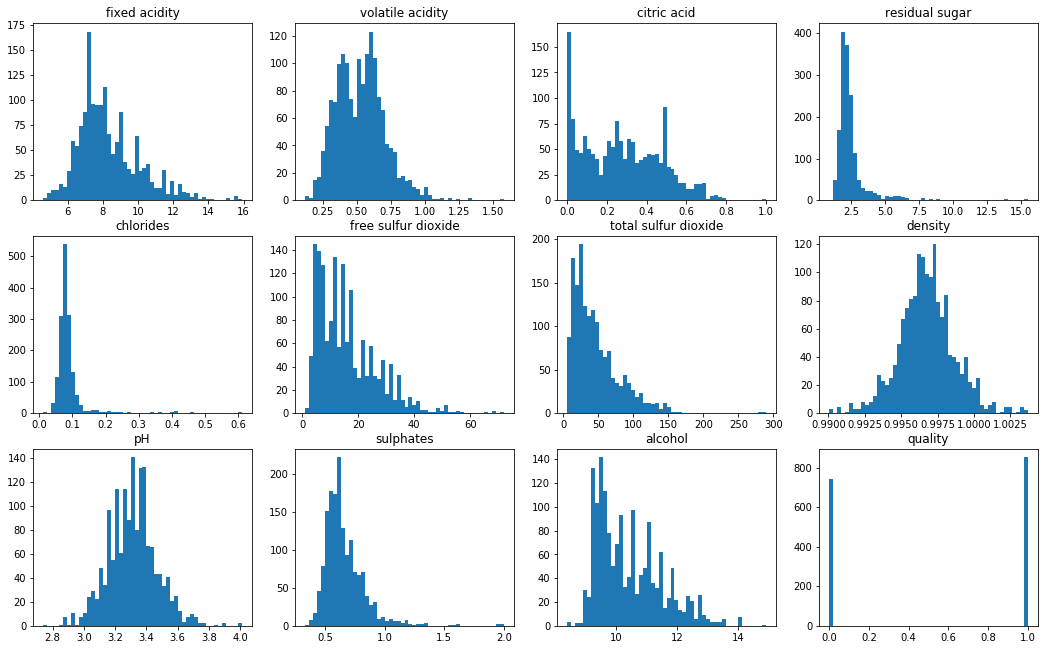
\includegraphics[width=240pt]{./img/wine_distribution.png}
\section{Results}


\section{Discussion and Conclusion}

\section{\label{sec:level1}Statement of Contribution}
Tianzhu Fu: Primary role was to construct a clean breast cancer dataset and plot the distribution of different attribute levels given a feature. Also implemented Accuracy and F1-score to measure performance. Finally, contributed to writing the report. \linebreak

Wenzong Xia: Preprocessed the red wine dataset to eliminate peculiar entries and ensured data integrity. Analysed original dataset through computing statistics (mean, standard deviation, min, max, etc.) and plotting data distribution for each attribute. Investigated the best fitting distribution model for the features. Implemented 5-fold cross validation for running experiments. Investigated correlation between features of the datasets for better feature selection. Contributed to the relevant sections of the report.

\section{References}
\end{document}
%
% ****** End of file aipsamp.tex ******
